\documentclass[11pt,a4paper]{article}
\usepackage[utf8]{inputenc}
\usepackage{amsmath,amssymb}
\usepackage{mathptmx}
\usepackage[margin=22mm]{geometry}
\usepackage{enumitem,tikz}
\usetikzlibrary{arrows.meta}

\setlength{\parindent}{0pt}
\setlength{\parskip}{3pt}
\setlist[enumerate,1]{label=\arabic*.,leftmargin=7mm,
  itemsep=14pt,topsep=6pt,parsep=3pt}
\setlist[enumerate,2]{label=\alph*),leftmargin=7mm,
  itemsep=7pt,topsep=4pt,parsep=3pt}

\begin{document}
\thispagestyle{empty}

\begin{center}
  \textbf{\Large KUIS 1 Kalkulus 1 Kelas 105}\\[0.6cm]
  \textbf{\large Selasa, 29 September 2026}\\[3pt]
  \textbf{\large Waktu : 90 menit\qquad Sifat : Tertutup}\\[3pt]
  \rule{11cm}{0.8pt}\\[-8pt]
  \rule{11cm}{0.4pt}
\end{center}
\vspace{0.4cm}

\begin{enumerate}
  \item Selesaikan untuk $x$ dari pertidaksamaan
    $\displaystyle\frac{2}{|x+3|}<\frac1x$.

  \item
    \begin{enumerate}
      \item Diketahui garis $l_1:3x+4y=8$ dan garis
        $l_2:y=-\frac34x-5$. Hitung jarak antara $l_1$ dan $l_2$.
      \item Hitung jarak dari titik $P(2,-1)$ ke perpotongan antara garis
        $g_1:2x+y=3$ dan garis $g_2:x=\frac34y+1$.
    \end{enumerate}

  \item Buat grafik dari $y=|2x^2-1|+3$.

  \item Diberikan fungsi $f(x)=\sqrt{x-1}$ dan $g(x)=x+2$ pada interval
    $1\le x\le5$. Dapatkan fungsi komposisi $(f\circ g)(x)$ beserta domainnya.

  \item Dapatkan persamaan dari setengah bagian yang kiri dari lingkaran
    $x^2+y^2-4x+3=0$.
\end{enumerate}

\vspace{1cm}
\begin{center}
  \textbf{\large oO Kejujuran harus ditegakkan Oo}
\end{center}

\newpage
\begin{center}
  \textbf{\Large PEMBAHASAN KUIS 1}\\[3pt]
  \textbf{Kalkulus 1 Kelas 105}
\end{center}

\begin{enumerate}
  \item Kedua penyebut harus tidak nol, sehingga $x\ne-3$ dan $x\ne0$.
    Untuk setiap $x$ yang diperbolehkan, ruas kiri $\frac{2}{|x+3|}$ selalu positif.
    Agar ruas kiri lebih kecil dari $\frac1x$, ruas kanan juga harus positif.
    Jadi, kita harus memiliki $x>0$.
    Semua $x<0$ langsung tidak memenuhi pertidaksamaan.

    Karena $x>0$, maka $x+3>0$, sehingga $|x+3|=x+3$.
    Pertidaksamaan menjadi
    \[
      \frac2{x+3}<\frac1x.
    \]
    Kalikan kedua ruas dengan $x(x+3)$.
    Faktor ini positif, sehingga tanda pertidaksamaan tetap:
    \[
      2x<x+3\iff x<3.
    \]
    Gabungkan hasil $x<3$ dengan syarat sebelumnya, yaitu $x>0$:
    \[
      \boxed{\mathrm{HP}=\{x\in\mathbb{R}\mid0<x<3\}=(0,3)}.
    \]
    Nilai $0$ tidak termasuk karena membuat penyebut nol.
    Nilai $3$ juga tidak termasuk karena kedua ruas sama-sama bernilai $\frac13$.

  \item
    \begin{enumerate}
      \item Ubah kedua persamaan garis ke bentuk $Ax+By+C=0$:
        \[
          l_1:3x+4y-8=0,\qquad
          l_2:3x+4y+20=0.
        \]
        Persamaan kedua diperoleh dengan mengalikan
        $y=-\frac34x-5$ dengan $4$, lalu memindahkan semua suku ke satu ruas.
        Kedua garis memiliki gradien yang sama, yaitu $-\frac34$.
        Jadi, keduanya sejajar.

        Jarak dua garis sejajar diukur sepanjang arah yang tegak lurus terhadap keduanya.
        Jika koefisien $A$ dan $B$ sudah sama, rumus jaraknya adalah
        \[
          d=\frac{|C_2-C_1|}{\sqrt{A^2+B^2}}.
        \]
        Masukkan $A=3$, $B=4$, $C_1=-8$, dan $C_2=20$:
        \[
          d=\frac{|20-(-8)|}{\sqrt{3^2+4^2}}
            =\frac{28}{\sqrt{25}}=\boxed{\frac{28}{5}}.
        \]

      \item Cari titik potong kedua garis terlebih dahulu.
        Dari $g_1$, diperoleh $y=3-2x$.
        Sementara itu, persamaan $g_2$ dapat ditulis sebagai $4x-3y=4$.
        Substitusikan nilai $y$ dari $g_1$ ke $g_2$:
        \begin{align*}
          4x-3(3-2x)&=4,\\
          4x-9+6x&=4,\\
          10x&=13\quad\Longrightarrow\quad x=\frac{13}{10}.
        \end{align*}
        Masukkan kembali ke $y=3-2x$:
        \[
          y=3-2\left(\frac{13}{10}\right)
           =\frac{30}{10}-\frac{26}{10}=\frac25.
        \]
        Jadi, titik potongnya adalah $Q(\frac{13}{10},\frac25)$.
        Gunakan rumus jarak dua titik untuk menghitung jarak dari $P$ ke $Q$:
        \begin{align*}
          PQ&=\sqrt{\left(\frac{13}{10}-2\right)^2
                    +\left(\frac25-(-1)\right)^2}\\
            &=\sqrt{\left(-\frac7{10}\right)^2+\left(\frac75\right)^2}
             =\sqrt{\frac{49}{100}+\frac{196}{100}}\\
            &=\sqrt{\frac{245}{100}}=\boxed{\frac{7\sqrt5}{10}}.
        \end{align*}
    \end{enumerate}

  \newpage
  \item Mulai dari parabola $y=2x^2-1$.
    Nilai di dalam mutlak berubah tanda saat
    \[
      2x^2-1=0\iff x^2=\frac12\iff x=\pm\frac1{\sqrt2}.
    \]
    Jika $|x|\ge\frac1{\sqrt2}$, nilai $2x^2-1$ tak negatif, sehingga tetap.
    Jika $|x|<\frac1{\sqrt2}$, nilainya negatif, sehingga tandanya dibalik.
    Setelah ditambah $3$, diperoleh bentuk potongan
    \[
      \boxed{y=|2x^2-1|+3=
      \begin{cases}
        2x^2+2, & x\le-\frac1{\sqrt2}\ \text{atau}\ x\ge\frac1{\sqrt2},\\[4pt]
        4-2x^2, & -\frac1{\sqrt2}<x<\frac1{\sqrt2}.
      \end{cases}}
    \]
    Secara geometris, bagian grafik $y=2x^2-1$ yang berada di bawah sumbu-$x$
    dipantulkan ke atas oleh nilai mutlak.
    Kemudian seluruh grafik digeser $3$ satuan ke atas.

    Di bagian tengah, grafiknya adalah parabola $y=4-2x^2$ yang terbuka ke bawah.
    Di bagian luar, grafiknya mengikuti $y=2x^2+2$ yang terbuka ke atas.
    Kedua bagian menyambung pada $(-\frac1{\sqrt2},3)$ dan $(\frac1{\sqrt2},3)$.
    Beberapa titik bantu adalah
    \[
      \begin{array}{c|ccccc}
        x & -1 & -\frac1{\sqrt2} & 0 & \frac1{\sqrt2} & 1\\ \hline
        y & 4 & 3 & 4 & 3 & 4
      \end{array}
    \]
    Fungsi ini simetris terhadap sumbu-$y$ karena hanya memuat $x^2$.
    Sketsanya berbentuk seperti huruf W, dengan dua titik minimum bernilai $3$.

    \begin{center}
      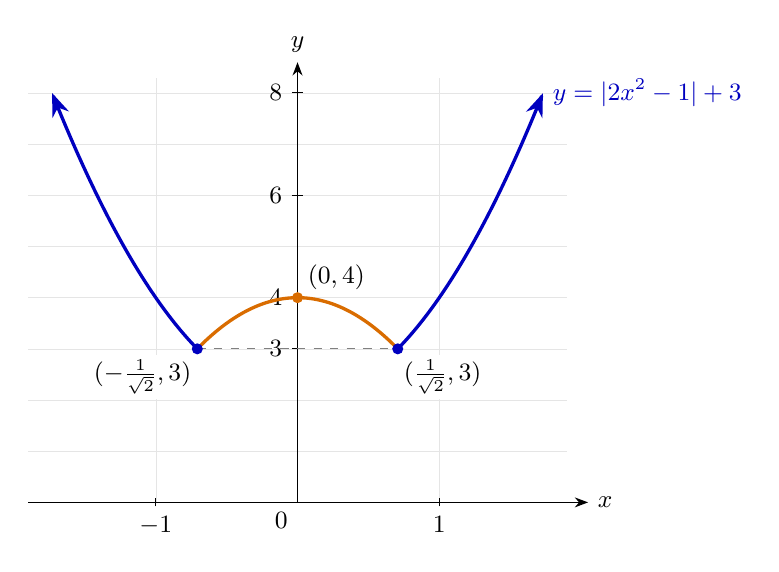
\begin{tikzpicture}[x=1.8cm,y=0.65cm,>=Stealth,font=\small]
        \draw[gray!20,very thin,step=1] (-1.9,0) grid (1.9,8.3);
        \draw[->] (-1.9,0)--(2.05,0) node[right] {$x$};
        \draw[->] (0,0)--(0,8.6) node[above] {$y$};
        \node[below left] at (0,0) {$0$};
        \foreach \x in {-1,1} {
          \draw (\x,-0.08)--(\x,0.08);
          \node[below] at (\x,-0.08) {$\x$};
        }
        \foreach \y in {3,4,6,8} {
          \draw (-0.04,\y)--(0.04,\y);
          \node[left] at (-0.04,\y) {$\y$};
        }
        \draw[gray,dashed] ({-1/sqrt(2)},3)--({1/sqrt(2)},3);
        \draw[blue!75!black,very thick,<-,domain=-1.732:-0.70710678,samples=100,smooth]
          plot (\x,{2*\x*\x+2});
        \draw[blue!75!black,very thick,->,domain=0.70710678:1.732,samples=100,smooth]
          plot (\x,{2*\x*\x+2});
        \draw[orange!85!black,very thick,domain=-0.70710678:0.70710678,samples=100,smooth]
          plot (\x,{4-2*\x*\x});
        \node[right,blue!75!black] at (1.732,8) {$y=|2x^2-1|+3$};
        \fill[blue!75!black] ({-1/sqrt(2)},3) circle (2pt);
        \fill[blue!75!black] ({1/sqrt(2)},3) circle (2pt);
        \fill[orange!85!black] (0,4) circle (2pt);
        \node[below left,fill=white,inner sep=2pt] at ({-1/sqrt(2)},2.9)
          {$(-\frac1{\sqrt2},3)$};
        \node[below right,fill=white,inner sep=2pt] at ({1/sqrt(2)},2.9)
          {$(\frac1{\sqrt2},3)$};
        \node[above right,fill=white,inner sep=1pt] at (0.05,4.1) {$(0,4)$};
      \end{tikzpicture}
    \end{center}
    Domain grafik adalah $\mathbb{R}$.
    Karena nilai mutlak selalu tak negatif, nilai $y$ selalu memenuhi $y\ge3$.
    Jadi, range-nya adalah $[3,\infty)$, dan grafik tidak memotong sumbu-$x$.

  \newpage
  \item Komposisi $(f\circ g)(x)$ berarti nilai $g(x)$ dimasukkan ke fungsi $f$.
    Karena $f(u)=\sqrt{u-1}$ dan $g(x)=x+2$, maka
    \[
      (f\circ g)(x)=f(g(x))=\sqrt{g(x)-1}
        =\sqrt{(x+2)-1}=\boxed{\sqrt{x+1}}.
    \]
    Interval $[1,5]$ pada soal dipakai sebagai domain kedua fungsi, yaitu
    $D_f=D_g=[1,5]$.
    Domain komposisi harus memenuhi dua syarat:
    \[
      D_{f\circ g}=\{x\in D_g\mid g(x)\in D_f\}.
    \]
    Pertama, masukan $x$ harus berada dalam $D_g$, sehingga $1\le x\le5$.
    Kedua, keluaran $g(x)=x+2$ harus berada dalam $D_f$:
    \[
      1\le x+2\le5\iff-1\le x\le3.
    \]
    Kedua syarat harus dipenuhi sekaligus, sehingga ambil irisannya:
    \[
      \boxed{D_{f\circ g}=[1,5]\cap[-1,3]=[1,3]}.
    \]
    Pada domain ini, bagian di dalam akar $x+1$ juga selalu positif.
    Kedua batas termasuk karena $g(1)=3$ dan $g(3)=5$ masih berada dalam $D_f$.

    \textit{Catatan: jika interval $[1,5]$ hanya dimaksudkan untuk $g$,
    sedangkan $f$ memakai domain alami $[1,\infty)$, domain komposisinya menjadi $[1,5]$.}

  \item Lengkapi kuadrat pada persamaan lingkaran:
    \begin{align*}
      x^2-4x+y^2&=-3,\\
      (x^2-4x+4)+y^2&=-3+4,\\
      (x-2)^2+y^2&=1.
    \end{align*}
    Jadi, pusat lingkaran adalah $(2,0)$ dan jari-jarinya $1$.
    Bagian kiri lingkaran terdiri dari titik-titik yang memenuhi $x\le2$.

    Nyatakan koordinat $x$ dalam bentuk $y$:
    \[
      (x-2)^2=1-y^2\quad\Longrightarrow\quad x-2=\pm\sqrt{1-y^2}.
    \]
    Karena bagian kiri memiliki $x-2\le0$, pilih tanda negatif:
    \[
      \boxed{x=2-\sqrt{1-y^2},\qquad -1\le y\le1}.
    \]
    Batas $y$ berasal dari syarat akar $1-y^2\ge0$.
    Persamaan ini menghasilkan $1\le x\le2$, sesuai bagian kiri lingkaran.
    Titik ujungnya adalah $(2,-1)$ dan $(2,1)$, sedangkan titik paling kirinya $(1,0)$.

    \begin{center}
      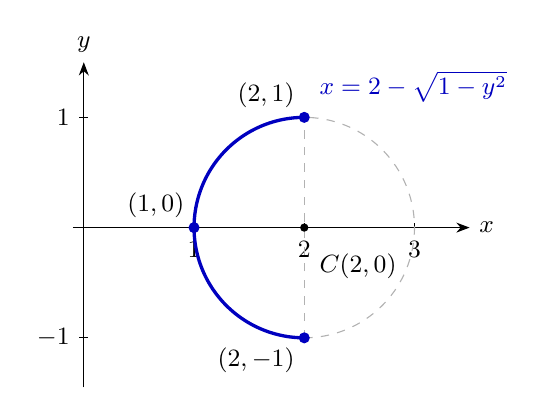
\begin{tikzpicture}[x=1.4cm,y=1.4cm,>=Stealth,font=\small]
        \draw[->] (-0.1,0)--(3.5,0) node[right] {$x$};
        \draw[->] (0,-1.45)--(0,1.5) node[above] {$y$};
        \foreach \x in {1,2,3} {
          \draw (\x,-0.04)--(\x,0.04);
          \node[below] at (\x,-0.04) {$\x$};
        }
        \foreach \y in {-1,1} {
          \draw (-0.04,\y)--(0.04,\y);
          \node[left] at (-0.04,\y) {$\y$};
        }
        \draw[gray!60,dashed,domain=-90:90,samples=100,smooth]
          plot ({2+cos(\x)},{sin(\x)});
        \draw[gray!60,dashed] (2,-1)--(2,1);
        \draw[blue!75!black,very thick,domain=-90:90,samples=100,smooth]
          plot ({2-cos(\x)},{sin(\x)});
        \node[above right,blue!75!black] at (2.05,1.05) {$x=2-\sqrt{1-y^2}$};
        \foreach \p in {(1,0),(2,1),(2,-1)} {\fill[blue!75!black] \p circle (2pt);}
        \fill (2,0) circle (1.5pt);
        \node[above left] at (2,1) {$(2,1)$};
        \node[below left] at (2,-1) {$(2,-1)$};
        \node[above left] at (1,0) {$(1,0)$};
        \node[below right] at (2.05,-0.15) {$C(2,0)$};
      \end{tikzpicture}
    \end{center}
    Kurva biru menunjukkan setengah lingkaran yang diminta.
\end{enumerate}

\end{document}
